%!TEX root = ../dokumentation.tex

\chapter{Prozessdokumentation}



Zeitlicher Verlauf des Projektes\\
Schwierigkeiten/Probleme ⇒ Behebung/Umgang\\
Wichtige Entscheidungen\\
Beschreibung der durchgeführten MCI Methoden mit ihren Ergebnissen\\
Aktivitätenverteilung (Wer hat was gemacht?)\\
Projektplan (geplant ⇔ tatsächlich)\\
Ziel: nachvollziehbare Prozessqualität\\

Wenn zur Klärung von Problemen Meinungen von den Betreuern eingeholt 

\newpage

%!TEX root = ../dokumentation.tex

\section{Anfänglicher Projektstand}
Das \textbf{Find your Camp} Projekt, befasst sich mit der Entwicklung einer Smartphoneanwendung für Androidgeräte, als Verleihsystem von privaten Grundstücken als Unterkunft. Die erste Projektphase befasste sich dabei mit der Entwicklung eines Exposes und anschließender Konzepterarbeitung zur Ausgangsidee. Im Rahmen dieser Phase wurden vorhandene Alternativen am Markt untersucht, Alleinstellungsmerkmale und Risiken in Bezug auf die Anwendungsdomäne abgewogen und es fand eine thematische Einarbeitung in die Problemdomäne statt.\\
Der Beschäftigung mit MCI Aspekten folgte der Entschluss, das Vorgehen auf Basis des \textbf{Usage Centered Design} durchzuführen, da der Schwerpunkt des Projektes auf den Interaktionen der Anwender liegt und die erwartete Benutzergruppe nicht durch bestimmte Merkmale konkretisiert werden kann.\footnote{Konzeptseite 12}
Weiterhin fanden erste Auseinandersetzungen mit dem Nutzungskontext\footnote{ab Konzeptseite 18}, der Nutzungsmotivation und ersten Anforderungsanalysen statt.\\
Für die Umsetzung wurde eine Systemarchitektur unter Einbezug der Google Cloud angedacht und die erste Testphase über die Proof-of-Concepts\footnote{Konzeptseite 41} geplant.\\

Zur weiteren Projektephase wurden zudem 2 Meilensteine definiert. Die Bearbeitung des ersten Meilensteins, sah die Umsetzung der weiteren MCI Methoden und die Durchführung der Proof-of-Concepts vor, wie dem Auszug des Projektplans (Abb. \ref{fig:projektplan}) bei Konzeptabgabe zu entnehmen ist. Angedacht waren hierfür 3 Wochen Arbeitszeit, deren einzelnen Schritte nach und nach verfeinert werden.
\begin{figure}[H]
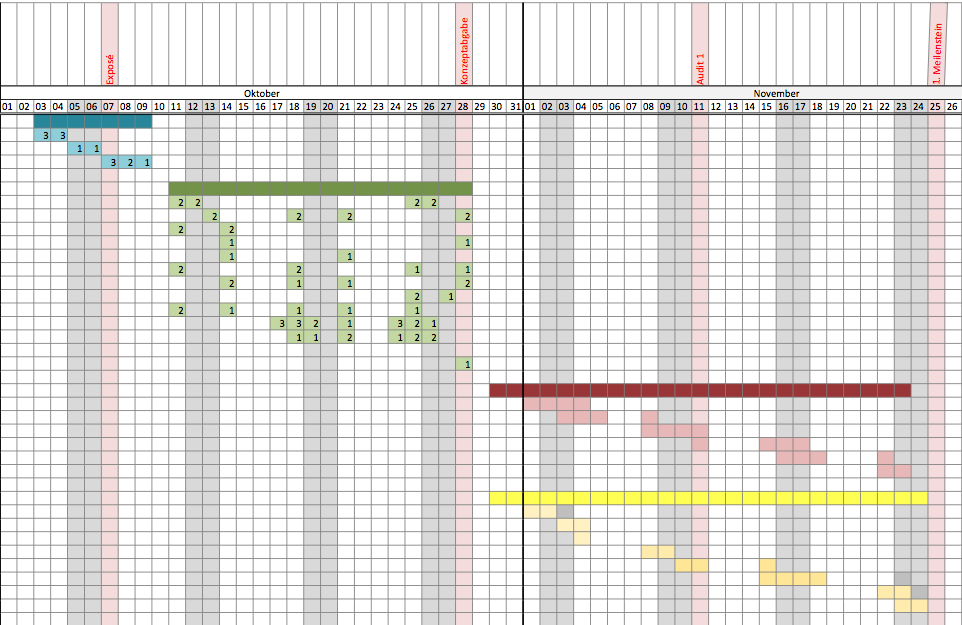
\includegraphics[width=1\textwidth]{./images/ausgangsplan.png}
\caption{Ausgangsplan bei Konzeptabgabe}
\label{fig:projektplan}
\end{figure}

Innerhalb welcher Zeitrahmen die einzelnen Arbeitsschritte letztendlich umgesetzt wurden, wird an gegeben Stellen deutlich gemacht.\\

\subsection{Konzeptüberarbeitungen}
Bevor mit der Dokumentation neuer Ergebnisse begonnen wurde, ging es um die Umsetzung des Konzeptfeedbacks und die Überarbeitung vorhandener Ausarbeitungen.\\
Damit die einzelnen Abschnitte inhaltlich etwas deutlicher aufeinander aufbauen, wurde die grundlegende Struktur des Dokumentes überarbeitet und das Geschäftsmodell sowie Zielhierachie als eigener Schwerpunkt herausgenommen. Die Abwägung des MCI Vorgehens wurde erweitert und an geeigneten Stellen präziser formuliert.\\

Erste Ansätze zum Geschäftsmodell wurden konkretisiert und mit Kennzahlen versehen. Die Vorgehensmöglichkeiten wurden dabei im Gespräch abgewogen und zu einem einheitlichen Modell zusammengefasst, anhand dessen eine Finanzierung als möglich erachtet wird. Die Zielhierachie wurde genauer auf das Projekt bezogen, da der vorherige Fokus zu wirtschaftlich und von langfristigen Zielen geprägt war.

\newpage
Ansätze zur Risikominimierung wurden ausführlicher und mit deutlicherem Bezug zum Konzept dokumentiert. Innherhalb der Anforderungsanalyse wurden nach eigenem Ermessen die funktionalen und qualitativen Anforderungen ausgebaut und zusätzlich erste organisatorische Anforderungen betrachtet.\\
Im WBA2 Teil, wurde das Kapitel zum Datenmodell erarbeitet und angedachte Proof-of-Concepts mit Bedeutung für das System genauer in Zusammenhang gebracht.\\

Für die Überarbeitung genannter Punkte, wurden im Vorfeld 1-2 weitere Arbeitstag eingeplant. Die letztendliche Arbeitszeit erstreckte sich jedoch auf eine gesamte Woche, was zur Folge hatte, dass der angesetzte Zeitrahmen der MCI Bearbeitungen verschoben werden musste. Der Grund der Überarbeitungsdauer liegt vor allem an der Bearbeitungstiefe, da gesamtes Konzept geprüft und wesentliche Aspekte weiter ausgearbeitet wurden. Kritisch für den Zeitplan wurde dies jedoch nicht angesehen, da die Überarbeitung auch Ergänzungen beinhaltet, die an anderer Stelle während der Dokumentation aufgetreten wären, jetzt jedoch im Konzept Einzug fanden.\\ Mit fortschreitender Projektzeit wurde deutlich, dass der erste gesetzte Meilenstein, bezogen auf die MCI Auseinandersetzung, mehr einer ersten Iterationsphase gleich kommt, als einer ausreichenden Betrachtung. Aufgrund des iterativen Charakters eines menschbezogenen Entwicklungsprojekts mit Evaluationen und Überarbeitungen der Ergebnisse, wurde die MCI Betrachtung über den gesamten Projektverlauf ausgelegt.



\newpage

%!TEX root = ../dokumentation.tex

\section{Ausarbeitung MCI}

Was sind die Entwicklungsziele für das interaktive System? X\\
Wer sind die Benutzer? X\\
Was sind die user needs? X\\
Was sind die funktionalen und qualitativen Anforderungen; welche Rahmenbedingungen existieren? X\\
Welche organisatorischen Anforderungen liegen vor x\\
Wie soll methodisch im Projekt vorgegangen werden? Wie werden die beiden Perspektiven ("MMA" und "MCI") in EINEM Projekt systematisch und strukturiert berücksichtigt? Vorgehensmodelle? Begründung und kritische Diskussion der Alternativen notwendig. x\\
Welches sind die Aufgaben, welche Struktur weisen sie auf und in welchen Beziehungen stehen die Aufgaben zueinander?\\
Wie sieht ein valides Modell des Nutzungskontextes aus? x\\
Welche Metaphern und Paradigmen liegen in der Domäne vor?\\
Welches ist das konzeptuelle Modell für das präskriptive Aufgabenmodell? \\
Welche Bezüge existieren bzgl. der Entwicklungsziele?\\
Welche alternativen konzeptuellen Modelle wurden entwickelt und wie wurde mit Design-Alternativen verfahren?\\
Welche Interaktions-Paradigmen, -Modi und -Stile wurden in Betracht gezogen? Erörterung notwendig.\\
Welche Prototypen wurden entwickelt, was zeichnet die verschiedenen Prototypen-Alternativen aus und wie wurde eine Synthese der Alternativen erreicht?\\
Nach welchen Kriterien wurden die Evaluation-Methoden und -Techniken ausgewählt?\\
Welches sind die Evaluationsergebnisse, welchen Erfüllungsgrad der Entwicklungsziele weist der finale Prototyp auf?\\
Welche Konsequenzen für das Redesign ergeben sich?\\
Wie sehen die weiteren Iterationen aus?\\

\newpage

%!TEX root = ../dokumentation.tex

\section{Weiterführende Benutzermodellierung}
Innerhalb der Konzeptphase wurde bereits der Grundstein zur Benutzermodellierung gelegt. Bezogen auf die Zieldomäne fand eine Identifikation vorhandener Stakeholdergruppen samt Einordnung statt. Für die weitere Auseinandersetzung geht es nun darum, die einzelnen Benutzergruppen genauer zu analysieren und entsprechende User Profiles zu entwickeln, um die Anwender genauer bestimmten zu können. Daraufhin aufbauend sollen Beispielpersona erstellt werden, da diese innerhalb des Designprozesse geeigneter sind um Interaktionsprozesse nachvollziehbarer zu gestalten. Der Vorteil von Persona gegenüber User Profiles liegt darin, dass kognitive Vorgänge durch die “Modellierung” einer Person mit Hintergrundinformationen präziser zu erreichen sind. Zudem ist es während der Entwicklung (vorerst) nicht möglich mit realen Personen zusammen zu arbeiten. 

Auch wenn der Fokus des Usage Center Designs auf der eigentlichen Interaktion liegt, sollte diese Modellierungstiefe erreicht werden, da innerhalb des Verleihprozesses unterschiedliche Anwendertypen auftreten können mit eigenen (moralischen) Ansichten zum Shared Economy Konzept. Speziell bezogen auf eine Zielgruppe, die ihr Grundstück nur unter bestimmten Sicherheitsaspekten verleihen würde, kann die Auseinandersetzung neue Erkenntnisse zu geforderten Funktionalitäten und Restriktionen liefern.

\subsection{User Profiles}
Entsprechend der Stakeholderanalyse\footnote{Konzeptkapitel 3.1 Seite 14} und der genaueren Benutzerbetrachtung im Rahmen des Nutzungskontexts\footnote{Konzeptkapitel 3.2 Seite 18}, geht es im nächsten Detaillierungsgrad um die Entwicklung von User Profiles. Dabei werden entsprechend der Stakeholdergruppen charakterisierende Merkmale analysiert.\footnote{Entsprechend Draft zur MCI S.376}\\
Vorerst stellte sich die Frage, für welche Stakeholdergruppen die weitere Modellierung den größten Nutzen hat. Da innerhalb des Entwicklungsprozesses speziell auf die Bedürfnisse der Anwender eingegangen wird, erscheint es am sinnvollsten die Usergruppen zu betrachten, die direkt mit dem System agieren. Dazu zählen vorallem die primary und secundary user. Für die tertiären user, die in ihrer Funktion hauptsächlich als Interessenten oder Richtungsgeber tätig sind, soll dieser Schritt nicht im Detail durchgeführt werden. (Feedback abwarten) Als potentielle Stakeholder dieser Klasse wurden beispielsweise andere Unterkunftsanbieter oder die Stadt, als Interessent durch den Tourismus, identifiziert. Da diese Gruppen grundsätzlich eher konzeptioneller Natur sind, spielen sie für die Entwicklung keine tragende Rolle.\\

Zuerst werden die primary user untersucht. Dazu gehören die Reisenden als Mieter und die Grundstücksbesitzer als Vermieter, die direkt mit dem System interagieren.

\newpage
\subsubsection{User Profile 1: Mieter (primary user)}
\begin{itemize}
   \item 
   \textbf{Demografisch:} Das Mindestalter beträgt 18 Jahre, es gibt kein obere Altersgrenze. Kernzielgruppe wird auf 18 - 40 Jahre geschätzt. Können prinzipiell aus jedem Land stammen, Wohnort ist für Reisende nicht relevant, müssen nur Anwedung und Internetzugang besitzen. Grundsätzlich also auch Reise aus verschiedenen Ländern möglich.

   \item 
  \textbf{Sozialökonomisch:} Mieter stammen aus unterschiedlichen Einkommensklassen, die Kernzielgruppe wird aus einkommensschwächeren bzw. finanzbewussten Leuten geschätzt (größte Motivation). 
   Aufgrund ihres Alters (und geschätzten Einkommens) wird nur ein ein geringer Teil auch Eigentumsbesitzer sein. Grundstücksbesitz eher bei Verwandten oder in Form von Gärten.

   \item 
   \textbf{Kultureller Hintergrund:} Können unterschiedlichen kulturellen Hintergrund haben, Kernzielgruppe wird jedoch in Deutschland oder dem europäischen Umfeld aufgewachsen sein. Sprachliche Kenntnisse im wesentlichen Deutsch und Englisch.

   \item
  \textbf{Physiologisch:} Aufgrund der Reisetätigkeit als Backpacker/Wanderer/Camper ist das Mindestmaß, dass die Anwendung benutzt werden kann; Grundsätzlich ist jeder potentieller Nutzer, daher sollte mit Beeinträchtigungen gerechnet werden. Auditive und visuelle Beeinträchtigungen sind möglich. Der Großteil besitzt aber keine schwerwiegenden Beeinträchtigungen, die speziell fokusiert werden müssen.

   \item 
   \textbf{Einstellung:} Vermutlich sozial offenere Menschen (vertrauensvolle), naturgebunden und reisefreudig. Haben keine Angst im Umgang mit der Technologie und der Thematikbezogenen Interaktion mit fremden Mietern als Vermieter. Auf ihrer Reise können sie zeitlich stark gebunden sein.

   \item 
  \textbf{Domänenkenntnisse:} Mit Erfahrung der Campingdomäne kann gerechnet werden, muss aber nicht zwangsläufig vorhanden sein.
   Erfahrene Leute in diesem Bereich, haben eventuell schon Kontakt mit Internetportalen gehabt, aber nicht zwangsläufig mit einer Smartphoneanwendung (für diesen Fall) gearbeitet.
   Innerhalb des Shared Economy haben sie eventuell schon Erfahrung in alternative Varianten wie Couchsurfing.

   \item
   \textbf{Technologieerfahrung:} Kenntnisse im Umgang mit dem Smartphone und der grundlegenden Anwendung von Applikationen kann vorausgesetzt werden.

   \item
  \textbf{verfügbare Technologien:} Besitzen ein Android Handy mit entsprechender Anwendung und Internetzugang. Dabei über Netzanbieter oder lokalen Hotspots.

   \item
   \textbf{Motivation:} Komfortabilität des Smartphones nutzen, Suchanfrage vereinfachen, Kosteneinsparung gegenüber gängigen Varianten, sozialer Kontakt-

   \item
   \textbf{Aufgabe:} Suchen einer geeigneten Unterkunft mit Anreise, Absprache und Bezahlung.
   
\end{itemize}
Wahrscheinlichkeit das diese Anwendergruppe auftritt: sicher


\newpage
\subsubsection{User Profile: Vermieter (primary user)}
\begin{itemize}
   \item 
   \textbf{Demografisch:} Das Mindestalter beträgt 18 Jahre, es gibt kein obere Altersgrenze. Kernzielgruppe wird auf 25 - 55 Jahre geschätzt. Wohnort innerhalb Deutschlands (bzw. Lage des Grundstückes) und ein bedeutender Teil lebt mit ihrer Familie (mit Kindern). Als Hilfsperson des secondary User auch mit jüngerem Alter möglich, dabei jedoch mit Registrierung des gesetzlichen Eigenstümers.

   \item 
  \textbf{Sozialökonomisch:} Jede Einkommensklasse möglich, sind im Besitz von Eigentum und stehen wahrscheinlich im Berufsleben. (Wenn sie als Zwischenperson agieren, Familienmitglied oder Bekannte.)

   \item 
   \textbf{Kultureller Hintergrund:} Großteil in Deutschland aufgewachsen und an Werte angepasst. Deutsche Sprachkenntnisse garantiert vorhanden, Englisch bei vielen.

   \item
  \textbf{Physiologisch:} Verschiedenste Beeinträchtigungen können auftreten, auch hier kein spezieller Fokus auf einzelne Einschränkungen.

   \item 
   \textbf{Einstellung:} Können unterschiedliche Einstellungen gegenüber dem Sharing Prinzip besitzen. Eventuell kein Interesse an sozialem Kontakt, auf geschäftlicher Ebene angesiedelt. Prinzipiell keine Angst im Umgang mit der Technologie, wobei Erfahrung nicht voraussgesetzt werden kann. Legen besonders Wert auf Datensicherheit.

   \item 
   \textbf{Domänenkenntnisse:} Können Erfahrung durch ähnliche Konzepte haben, grundsätzlich aber auch der erste Kontakt innerhalb der Anwendung möglich. Kenntnisse zur Vermietung mit rechtlichen Richtlinien sind ebenfalls nicht zwingend vorhanden, auch Erfahrung beim Camping/ Sharing Konzepten kann nicht vorausgesetzt werden.

   \item
   \textbf{Technologieerfahrung:} Erfahrung in der Benutzung eines Smartphones, tieferfreifendes, technisches Verständnis nicht zwangsläufig ausgeprägt.

   \item
   \textbf{verfügbare Technologien:} Smartphone mit Android und Anwendung, Internetzugang.

   \item
   \textbf{Motivation:} Finanzieller Anreiz wie Deckung möglicher Grundstückskosten oder für zusätzliches Einkommen. Dazu kommt soziale Erfahrung und Motivation zum Teilen/ Unterstützen.

   \item
   \textbf{Aufgabe:} Bekanntmachen des Angebotes für Mieter, Erfüllen der angedachten Vorraussetzungen des Reisenden.
   
\end{itemize}
Wahrscheinlichkeit das diese Anwendergruppe auftritt: sicher


\newpage
Folgendes User Profil befasst sich mit Grundstücksbesitzern, die selbst nicht mit der Technologie umgehen können oder wollen, dennoch bereit sind ihr Grundstück zu vermieten.
Die Mietobjektanzeige und Kontaktaufnahme wird dabei von einem weiteren Familienmiglied oder Bekannten in der stellvertretenden Rolle des primary users durchgeführt.\\

\subsubsection{User Profile: Zwischenperson für Vermieter (secondary user)}
\begin{itemize}
   \item 
   \textbf{Demografisch:} Mindestalter über 18 Jahre, Kernzielgruppe: 50 - 80 Jahre.  

   \item 
  \textbf{Sozialökonomisch:} Finanziell gefestigt, müssen nicht mehr im Berufsleben stehen. 

   \item 
   \textbf{Einstellung:} Erfahrene Menschen mit gefestigten Ansichten und Lebenserfahrungen. Einstellung oftmals fixiert und schwer beeinflussbar, daher Motivation schwer zu vermitteln.
   Stehen Technologie oftmals desinteressiert oder kritisch gegenüber. Technologieängste bei Vielzahl vorhanden.

   \item 
   \textbf{Domänenkenntnisse:} Haben eventuell Erfahrung in der Vergangenheit durch ähnliche Konzepte gehabt und konnten daher Interesse als Vermieter gewinnen.

   \item
   \textbf{Technologieerfahrung:} Nicht zwingend vorhanden. 

   \item
   \textbf{verfügbare Technologien:} Sind nicht im direkten Besitzer der Technologien, daher auf andere Besitzer angewiesen.

   \item
   \textbf{Motivation:} Anbieten des Grundstücks zur Vermietung.

   \item
   \textbf{Aufgabe:} Weitergabe der Angaben und Informationen an primary user, stellen den Input bereit.
   
\end{itemize}
Wahrscheinlichkeit das diese Anwendergruppe auftritt: sehr gering


\newpage
TODO
\subsubsection{User Profile: Kooperationspartner (Werbe- oder Event-)}
\begin{itemize}
   \item 
   \textbf{Kultureller Hintergrund:} Kooperationspartner kann aus unterschiedlichen Ländern stammen, hat aber Bezug zum deutschen Markt oder dort stattfindende Events. Standort oder Unternehmen ist (zum Teil) in Deutschland angesiedelt oder wirbt auf dem deutschen Markt.

   \item
   \textbf{Auftreten:} Vorrangig Unternehmen die domänenspezifische Produkte verkaufen. Zusätzlich Eventpartner unterschiedlicher Art, wobei es nicht zwangsläufig der bestimmte Veranstaltungsort sein kann, sondern der Veranstalter. Organisiert in mittelgroßen bis großen Maßstäben.

   \item 
   \textbf{Domänenbezogenes:} Werbeprodukt mit Relevanz zur Campingdomäne, Eventpartner mit Relevanz für entsprechenden Standort. Können bereits Kooperationserfahrung mit anderen Anbietern der Domäne haben. Definitive Erfahrung im relevanten Marketing.

   \item
   \textbf{Einstellung:} Sehen Applikationen und In-App Werbung als lokrative Werbemöglichkeit und haben die Anwender und Technologie als Werbeplattform erkannt. Setzen auf Werbung innerhalb dieser Technologie und haben keine Angst davor.

   \item
   \textbf{Motivation:} Werben bei einer starken Kernzielgruppe; Wahrscheinlichkeit, dass Anwender eher angesprochen werden als durch den "öffentlichen" Werbeweg ist relativ hoch. Zielgruppe jedoch bedeutend kleiner als bei Fernseh- oder Straßenwerbung
   
\end{itemize}
Wahrscheinlichkeit das diese Anwendergruppe auftritt: mittel - hoch

TODO Sonstige?\\
Primary\\
Mitarbeiter (Support)\\
Stadt\\
Konkurrierende Unterkunftsanbieter\\
Entwickler


\newpage
\subsection{Persona}
Aufbauend auf den entwickelten User Profiles, werden im nächsten Schritt Beispielpersona entwickelt, die Vetreter der einzelnen Stakeholdergruppen darstellen. Ziel ist der Aufbau eines Portfolios, in welchem die zuvor identifizierten Charakteristiken weitestgehen abgedeckt werden.

\textbf{Persona 1: Mathias Schmidt}\\
Status: primäry user (Mieter)\\

Alter: 40 \\
Wohnort: München, verheiratet\\
Familenstand: verheiratet, 1 Sohn Tim Schmidt (15)\\
Beruf: Mechaniker\\
Beeinträchtigungen: Sehschwäche (Brillenträger) \\

Mathias ist 40 Jahre alt und leidenschaftlicher Mechaniker. Neben seiner Arbeit betreibt er zum Ausgleich viel Sport und ist ein naturgebundener Mensch.
Er ist sehr offen und kontaktfreudig gegenüber anderen Leuten. In seinen 20er Jahren ist er oft verreist und investierte sein Einkommen in diese Beschäftigung. Dadurch konnte er sich die Englische Sprache beibringen, die im Laufe der Zeit jedoch etwas an Übung verloren hat. Seit dem muss er für seine Familie sorgen und schafft es aus beruflichen Gründen oftmals nicht längerfristig Urlaub zu bekommen und viel zu verreisen.\\

Er hat keine Erfahrung mit Couchsurfing oder Ähnlichem, diese Art des Reisens ist ihm jedoch nicht fremd. Er selbst konnte auf diese Art bisher keine Reise durchführen, da er den Fokus auf seine Familie legt.
Was Technologie angeht ist er weitestgehend interessiert am derzeitigen Stand, verfolgt jedoch keine spezifischen Nachricht und nimmt Informationen eher durch Zufall auf. Mit Computern und seinem Smartphone kann er sicher umgehen. Sein berufliches Ziel für die Zukunft ist weiterhin gesichertes Einkommen, eine höhere Karrie strebt er nicht an, da er mit seinen aktuellen Umständen soweit zufrieden ist. Privat würde er gerne mehr Zeit mit seinem Sohn investieren, schafft oftmals aber nur spontane Kurzausflüge, die finanziell nicht zuviel fordern.\\

Da er kurzfristig Überstunden absetzen konnte, plant er für die nächste Woche spontan eine Fahrradtour mit seinem Sohn. Ein Arbeitskollege berichtete ihm von seiner vergangengen Deutschlandreise, bei der er günstige Schlafplätze bei privaten Vermietern gefunden hat. Nach einer Suche im Internet stellt er fest, dass gängige Hotels und Unterkünfte zu teuer sind und kein Campingplatz auf seiner Reiseroute zu finden ist. Nach kurzer Recherche stößt er auf die Find your Camp Anwendung.
Er registriert sich dort als Mieter und verifiziert sich im Anschluss.



\newpage
\textbf{Persona 2: Christine Bayer }\\
Status: primary user (Mieter)\\

Alter: 21\\
Wohnort: Köln\\
Familenstand: ledig\\
Beruf: Journalismus Studentin\\
Beeinträchtigungen: - \\

Christine ist 21 Jahre, stammt aus Köln und möchte in ihren Semesterferien als Backpackerin durch ganz Europa reise.
Neben ihrer Tätigkeit als Student, verdient sie ihr Geld mit einem Nebenjob als Kellnerin und erhält zudem Bafög.
Sie interessiert sich besonders für Kulturen und Fotografie. Technik nimmt sie eher nebenläufig war, ist sicher im Umgang mit ihrem Computer und besitzt ein aktuelles Smartphone.
Privat erhofft sie sich nach dem Studium eine Karriere als freue Journalistin und sieht ihr Berufsfeld vorallem im Ausland.

Bereits im letzten Jahr unternahm sie einen Kurzaufenthalt in Berlin und nutzte dabei das Couchsurfing Portal um eine Unterkunft zu finden. Auch wenn sie sich mit ihrem Gastgeber gut verstand, empfand sie es etwas befremdlich permanent auf jemand anderen angewiesen zu sein. Dieses Mal ist sie mit einer guten Freundin unterwegs und gemeinsam beginnen sie ihre Reise Richtung Süddeutschland. Da sie für einen längeren Zeitraum unterwegs sind, sind sie auf günstige Angebote gewiesen. Hotels kommen daher nicht in Frage und Hostels nur in Ausnahmefällen. Da sie im Sommer verreisen nehmen sie leichte Zeltausrüstung mit und können zur Not auch im freien im Übernachten. Bei der Suche nach Anwendungen für ihre Reise, stößt sie durch Zufall auf die Find your Camp Anwendung.



\newpage
\textbf{Persona 3: Karin Schultz}\\
Status:primary user (Vermieter)\\

Alter: 32\\
Wohnort: Gummersbach\\
Familenstand: vergeben, 1 Kind\\
Beruf: Grundschulehrerin\\
Beeinträchtigungen: Sehschwäche\\

Karin ist 32 Jahre und lebt seit ihrer Geburt in Gummersbach. Sie lebt gemeinsam mit ihrem Freund und deren gemeinsamen Tochter im Haus ihrer Eltern. Aus Platzgründen stellt diese kein Problem dar.
Als Grundschullehrin ist sie sehr offen und kontaktfreudig. Während ihrer Studienzeit verreiste sie gerne und absolvierte ein Teil ihres Studium im Ausland, wodurch sie viele Bekanntschaften schloss.
Seit der Geburt ihrer Tochter ist sie nicht mehr verreist und verbrachte viel Zeit mit ihrer Familie. \\

Über eine Kollegin erfährt sie von der Find your Camp Anwendung. Seit 1 Monat seie sie dort angemeldet und bietet ihren Garten zur Untermiete an. Neulich hatte sie Besuch von 2 Studenten die auf der Durchreise von Leipzig nach Amsterdam waren und die ganze Vermietung bereitete ihr, bis auf eine einmalige registrierung, kaum Aufwand.\\

Da Karins Familie ein Haus mit großem Grundstück besitzt, dass sie aus zeitlichen Gründen eher vernachlässigte, beschließt sie sich, ebenfalls als Vermieterin anzumelden. Sie erhofft sich damit, neben einem kleinen finanziellen Gewinn vorallem Kontakt zu netten Leuten und das Gewinnen neuer Erfahrungen.

\newpage
\textbf{Persona 4: Wolfgang Ehrlichmann}\\
Status: primary user (Vermieter)\\

Alter: 52\\
Wohnort: Gummersbach\\
Familenstand: verheiratet, 2 Kinder\\
Beruf: Zahnarzt\\
Beeinträchtigungen: Farbschwäche\\

Wolfgang ist 52 Jahre alt, studierte Zahnmedizin in Hamburg und heiratete mit 36 seine Frau Tina. Als gebürtige Gummersbacherin, wollte sie dort weiterhin leben, wodurch er in ihre Heimat zog.
Dort baute er sich eine kleine Praxis auf und lebt mit gesichertem Einkommen in einem Einfamilienhaus. Ihre beiden Kinder studieren derzeit, sind sehr aktiv und an neuen Erfahrungen interessiert.
Über sie erfährt von den Reisearten der Shared Economy und steht dem ganzen eher kritisch gegenüber. Er selbst könnte sich nicht vorstellen bei Fremden in der Wohnung zu übernachten. \\
Da er mit dem Computer nur die wesentlichen Aufgaben für seinen Alltag bewältigt und ansonsten zufrieden ist mit den Dingen an die er gewohnt ist, sieht er keinen direkten Mehrwert am Internet und diversen Social Media Portalen.
Auch auf seinem Smartphone reichen ihm die üblichen Anwendungen wie Kalender und Email, um den Alltag zu bewältigen.\\

Nach mehreren Gesprächen mit seinen Kindern, konnten sie ihn davon überzogen, ihren Garten einmalig zur Probe zu vermieten. Er konnte letztendlich davon überzeugt werden, dass er seine Daten nicht öffentlich ins Internet stellen muss und vorher sieht wer zu ihm kommen möchte. Er selbst muss lediglich das Inserat erstellen, die Töchter übernehmen die eigentliche Vermietung und somit läuft für ihn alles ab, "wie bei einem Besuch von Freunden seiner Kinder".
Er erwartet sich als Gegenleistung für die Besuch jedoch eine Übernachtungsgebühr und das er den Garten in einem einwandfreien Zustand vorfindet.

\newpage
\textbf{Persona 5: Clara Hütt}\\
Status: primary user (für Vermieter)\\

Alter: 16\\
Wohnort: Neuwied\\
Beruf: Schülerin, 11. Klasse \\
Beeinträchtigungen: - \\

Clara ist 16 Jahre alt und Schülerin aus Neuwied. 
Sie lebt mit ihrer Familie in einem Mehrfamilienhaus. Ihr Mutter ist Bankkauffrau und ihr Vater Geschäftsmann. Beruflich ist er unterhalb der Woche oft auf Reise, wodurch sie mit ihrer Mutter oftmals alleine ist.
Sie ist sehr zurückhaltend, Interessiert sich für fremde Länder und alles was mit Medien zu tun hat. Sie ist mit dem Internet aufgewachsen und kann mit Technik problemlos umgehen.
Nach der Schule möchte sie gerne in Köln studieren und irgenwann mal im Ausland wohnen.\\
In ihrere Freizeit unternimmt sie viel mit Freunden. Früher als ihr Vater weniger verreisen musste, war sie mit ihrer Familie am Wochenende meistens im Garten und zeltete dort ab und an mit ihren Freundinnen.
Aus zeitlichen Gründen wird der Garten derzeit weniger genutzt und die Mutter steht daher vor der Entscheidung den Garten abzugeben, da ansonsten unnötiger finanzieller Aufwand ansteht.
Als sie von Find your Camp erfährt möchte sie versuchen die Kosten darüber zu decken. Da sie selbst kein Smartphone besitzt, bittet sie Clara darum, das Inserat für sie zu erstellen. Sie soll lediglich bei Angeboten bescheid geben und die Mutter übernimmt die weiteren Verpflichtungen. Als Belohnung erhält Clara einen Anteil der Gebühren.\\


TODO in einer weiteren Iteration neue Persona entwickeln mit weiteren Perspektiven zur Thematik.\\


Wer sind die Anwender, wie stehen sie zum System?\\


Role Model: user <-> system\\
role Model:: user roles, user role map zusammenspiel der user role\\
user role: abstraction needs, interests, expectations, behaviors, responsibilities (Wirfs Brock 1993, Software for Use S 79)\\



%Arbeit und Aufgabenmodellierung
\newpage

%!TEX root = ../dokumentation.tex

\section{Aufgabenmodellierung}

Was sind die Aufgaben die sie erreichen wollen?\\
Was benötigen sie vom System und wie sollte das organisiert sein?\\

use case methoden: allistar cockburn template \\
concrete use case, lockwood\\


-> User Role/ Use Cases speziell für usage centered	\\
task model essentiell use cases, use case map ale aufeinander\\

task Model: struktur der Aufgaben\\


\subsection{Essentiel Use Cases}
Funktionale Anforderungsermittlung, interaktion zwischen Anwender und System, sehr abstrakt, grober Überblick, technologie frei\\
Formal und an Reichhaltigkeit orientiert an Software for Use S. 105

\begin{table}[H]
\caption{\#1 Anwender bekanntmachen }
\centering
\begin{tabular}{l l}
\\ [-0.5ex]

\hline\hline
\\ [-0.5ex]
user intention & system responsibility
\\ [1.5ex]
\hline
\\ [-0.5ex]
Aktion auswählen 			& 											\\[1ex]
							& Optionen bekanntmachen, Wahl ermöglichen	\\[1ex]
Informationen angeben 		& 											\\[1ex] 
							& Informationen aufnehmen					\\[1ex]
							& Informationen präsentieren				\\[1ex]
Informationen bestätigen	& 											\\[1ex]
							& Bestätigung anbieten, bei Wahl akzeptieren \\[1ex]


\hline
\end{tabular}
\label{tab:anmelden}
\end{table}

\begin{table}[H]
\caption{\#2 Benutzerprofil verwalten }
\centering
\begin{tabular}{l l}
\\ [-0.5ex]

\hline\hline
\\ [-0.5ex]
user intention & system responsibility
\\ [1.5ex]
\hline
\\ [-0.5ex]
Aktion auswählen 			& 											 \\[1ex]
							& Optionen bekanntmachen, Wahl ermöglichen	 \\[1ex]
Identität bestätigen		& 											 \\[1ex]
							& Identität prüfen							 \\[1ex]
							& vorhandene Informationen präsentieren      \\[1ex] 
Informationen ändern 		& 											 \\[1ex] 
							& neue Informationen aufnehmen				 \\[1ex]
							& alte Informationen entfernen				 \\[1ex]
Informationen bestätigen	& 											 \\[1ex]
							& Bestätigung anbieten, bei Wahl akzeptieren \\[1ex]
\hline
\end{tabular}
\label{tab:profilbearbeiten}
\end{table}

\begin{table}[H]
\caption{\#3 Mietauftrag erstellen }
\centering
\begin{tabular}{l l}
\\ [-0.5ex]

\hline\hline
\\ [-0.5ex]
user intention & system responsibility
\\ [1.5ex]
\hline
\\ [-0.5ex]
Aktion auswählen 			& 											 \\[1ex]
							& Optionen bekanntmachen, Wahl ermöglichen	 \\[1ex]
Identität bestätigen		& 											 \\[1ex]
							& Identität prüfen							 \\[1ex]
Informationen anlegen 		& 											 \\[1ex] 
							& neue Informationen aufnehmen				 \\[1ex]
							& Informationen präsentieren				 \\[1ex]
Informationen bestätigen	& 											 \\[1ex]
							& Bestätigung anbieten, bei Wahl akzeptieren \\[1ex]

\hline
\end{tabular}
\label{tab:mietauftrag}
\end{table}

\begin{table}[H]
\caption{\#4 Mietobjekt finden }
\centering
\begin{tabular}{l l}
\\ [-0.5ex]

\hline\hline
\\ [-0.5ex]
user intention & system responsibility
\\ [1.5ex]
\hline
\\ [-0.5ex]
Aktion auswählen 			& 											 \\[1ex]
							& Optionen bekanntmachen, Wahl ermöglichen	 \\[1ex]
Mietauftrag bekanntmachen	& 											 \\[1ex]
							& vorhandene Mietaufträge präsentieren		 \\[1ex]
							& Option für neuen Mietauftrag anbieten      \\[1ex]
Anfrage bestätigen   		& 											 \\[1ex] 
							& Anfrage akzeptieren						 \\[1ex]
							& Anfrage bearbeiten \\[1ex]
Antwort erhalten			& 											 \\[1ex]
							& Akteur über Antwort informieren			 \\[1ex]

\hline
\end{tabular}
\label{tab:mietobjekt}
\end{table}

\begin{table}[H]
\caption{\#5 Mietanfrage beantworten }
\centering
\begin{tabular}{l l}
\\ [-0.5ex]

\hline\hline
\\ [-0.5ex]
user intention & system responsibility
\\ [1.5ex]
\hline
\\ [-0.5ex]
Mietanfrage bekommen 		& 											 \\[1ex]
							& neue Mietanfrage präsentieren				 \\[1ex]
Mietanfrage einsehen		& 											 \\[1ex]
							& Informationen präsentieren				 \\[1ex]
Mietanfrage beantworten  	& 											 \\[1ex] 
							& Auswahl anbieten							 \\[1ex]
							& nächsten Schritt anbieten					 \\[1ex]
Informationen mitteilen		& 											 \\[1ex]
							& vorhandene Informationen anzeigen			 \\[1ex]
							& Informationen vermitteln					 \\[1ex]


\hline
\end{tabular}
\label{tab:mietanfrage}
\end{table}

\begin{table}[H]
\caption{\#6 Bezahlung }
\centering
\begin{tabular}{l l}
\\ [-0.5ex]

\hline\hline
\\ [-0.5ex]
user intention & system responsibility
\\ [1.5ex]
\hline
\\ [-0.5ex]
Aktion auswählen	 		& 											 \\[1ex]
							& Option anbieten							 \\[1ex]
Identität bestätigen		& 											 \\[1ex]
							& Identität prüfen							 \\[1ex]
Mietauftrag wählen		  	& 											 \\[1ex] 
							& Mietaufträge präsentieren, Wahl ermöglichen\\[1ex]
Bezahlauftrag starten		& 											 \\[1ex]
							& relevante Informationen präsentieren		 \\[1ex]
							& Informationsaufnahme anbieten	     		 \\[1ex]
Auftrag bestätigen			&	     									 \\[1ex]
							& Bestätigung anbieten				   		 \\[1ex]
							& Ergebnis präsentieren			    		 \\[1ex]

\hline
\end{tabular}
\label{tab:statuscodes}
\end{table}

\newpage
\subsection{Concrete Use Case}
Ein use case erfasst eine Beziehung zwischen stakeholder und dem technischen Subsystem bzgl. des Verhaltens des technischen Subsys- tems. Es beschreibt das Verhalten des technischen Subsystems unter bestimmten Rahmenbedingungen als Antwort auf eine Anfrage des stakeholders (primary actor). Der primary actor iniziiert die Interak- tion, um ein Ziel zu erreichen.

\begin{table}[H]
\caption{Use Case\#1 Benutzer registrieren }
\centering
\begin{tabular}{l l}
\\ [-0.5ex]

\hline\hline
\\ [-0.5ex]
user intention & system responsibility
\\ [1.5ex]
\hline
\\ [-0.5ex]
Funktion zur Neuanmeldung auswählen 				& 												\\[1ex]
													& Funktion bereitstellen, die dies ermöglicht	\\[1ex]
													& Über Richtlinien hinweisen 					\\[1ex]
Kenntnissnahme zu Richtlinien bestätigen			& 												\\[1ex]
													& Bestätigung ermöglichen						\\[1ex]
Informationen eingeben 								& 												\\[1ex] 
Personeninformationen Name, Vorname, Gebdat etc. 	& 												\\[1ex] 
													& Eingabefelder bereitstellen, Informationen    \\[1ex]
													& aufnehmen, weitere Schritte ermöglichen		\\[1ex]
Korrektheit der Daten prüfen und bestätigen			& 												\\[1ex]
													& Funktion zur Bestätigung anbieten 			\\[1ex]
													& weitere Funktionalitäten anbieten, Mietobjekt \\[1ex]
													& anlegen oder Mietauftrag anlegen				\\[1ex]
													& Informationen zur Verifizierung senden		\\[1ex]
Profil verifizieren									& 												\\[1ex]
													& TODO verifizierungsschritte (extra Use Case?)	\\[1ex]


\hline
\end{tabular}
\label{tab:anmeldenUC}
\end{table}

\begin{table}[H]
\caption{Use Case\#2 Benutzerprofil verwalten }
\centering
\begin{tabular}{l l}
\\ [-0.5ex]

\hline\hline
\\ [-0.5ex]
user intention & system responsibility
\\ [1.5ex]
\hline
\\ [-0.5ex]
Funktion zur Verwaltung auswählen  	& 												 	\\[1ex]
									& Funktion bereitstellen, die dies ermöglicht	 	\\[1ex]
Identität bestätigen				& 											     	\\[1ex]
									& Identitätsabfrage einleiten und mit Eingabe    	\\[1ex]
									& prüfen, anschließend bereits vorhandene 		 	\\[1ex] 
									& Informationen anzeigen     				     	\\[1ex] 
Neuen Informationen eingeben 		& 											     	\\[1ex] 
									& neue Informationen über Eingabefelder aufnehmen, 	\\[1ex]
									& auf syntaktische Korrektheit prüfen				\\[1ex]
Neue Informationen abspeichern		& 											 		\\[1ex]
									& Funktion zum abspeichern anbieten					\\[1ex]
\hline
\end{tabular}
\label{tab:profilbearbeitenUC}
\end{table}

\begin{table}[H]
\caption{Use Case\#3 Mietauftrag erstellen }
\centering
\begin{tabular}{l l}
\\ [-0.5ex]

\hline\hline
\\ [-0.5ex]
user intention & system responsibility
\\ [1.5ex]
\hline
\\ [-0.5ex]
Funktion zum neuen Mietauftrag wählen 		& 												\\[1ex]
											& Funktion bereitstellen, die dies ermöglicht	\\[1ex]
Profil des Reisenden auswählen über den		& 												\\[1ex]
gemietet werden soll          				& 												\\[1ex]
											& Anmeldung mit Benutzerdaten ermöglichen		\\[1ex]
Organisatorische Informationen eintragen	& 											 	\\[1ex] 
											& Eingabefelder bereitstellen und 				\\[1ex]
											& Informationen aufnehmen 						\\[1ex]
Gewünschte Austattung auswählen				& 					 							\\[1ex]
											& Austattungsmerkmale anzeigen und 				\\[1ex]
											& Auswahl über Menü ermöglichen 				\\[1ex]
Informationen bestätigen und abspeichern 	& 												\\[1ex]
										 	& Funktion zum abspeichern anbieten 			\\[1ex]

\hline
\end{tabular}
\label{tab:mietauftragUC}
\end{table}

\begin{table}[H]
\caption{Use Case\#4 Mietobjekt finden }
\centering
\begin{tabular}{l l}
\\ [-0.5ex]

\hline\hline
\\ [-0.5ex]
user intention & system responsibility
\\ [1.5ex]
\hline
\\ [-0.5ex]
Funktion zur neuen Suchanfrage starten 	& 											 	\\[1ex]
										& Funktion bereitstellen, die dies ermöglicht	\\[1ex]
Passenden Mietauftrag zur Reise wählen	& 												\\[1ex]
										& Vorhandene angelegte Mietaufträge anzeigen	\\[1ex]
										& und Auswahl ermöglichen, Option zum anlegen   \\[1ex]
										& eines neuen Auftrags anzeigen					\\[1ex]
Suchanfrage ausführen 					& 												\\[1ex] 
										& Ausgewählten Auftrag anzeigen	und Suchanfrage	\\[1ex]
										& funktional ermöglichen, nach Bestätigung 		\\[1ex]
										& GPS Daten bestimmen und Anfrage weiterleiten.	\\[1ex]
										& Benutzer über getätigte Suche informieren		\\[1ex]
Rückmeldung zu vorhandenen Angeboten	& 												\\[1ex]
erhalten								& 												\\[1ex]
										& Wenn kein Angebot vorhanden ist, direkte		\\[1ex]
										& Rückmeldung. Ansonsten regelmäßige Abfrage 	\\[1ex]
										& an Server, ob Vermieter angenommen hat.		\\[1ex]
										& Meldung an Benutzer schicken bei Treffer 		\\[1ex]
										& nach Ablauf einer kritischen Zeit.				\\[1ex]
\hline
\end{tabular}
\label{tab:mietobjektUC}
\end{table}

\begin{table}[H]
\caption{Use Case\#5 Mietanfrage beantworten }
\centering
\begin{tabular}{l l}
\\ [-0.5ex]

\hline\hline
\\ [-0.5ex]
user intention & system responsibility
\\ [1.5ex]
\hline
\\ [-0.5ex]
Meldung über relevante Mietanfrage 	& 												\\[1ex]
erhalten 							& 												\\[1ex]
									& Mietauftrag empfangen und lokal matchen		\\[1ex]
									& bei Bestätigung Meldung mit Informationen		\\[1ex]
									& auf dem Display hervorheben, Benachrichtigen	\\[1ex]
Mieterdaten ansehen					& 											 	\\[1ex]
									& Reisedaten anzeigen: Datum Gruppengröße		\\[1ex]
									& Preisvorstellung, Anfragezeit					\\[1ex]
Mietanfrage beantworten  			& 												\\[1ex] 
									& Funktion anbieten zur Annahme oder Ablehnung 	\\[1ex]
									& der Anfrage, Meldung an Mieter schicken      	\\[1ex]
Annahme des Auftrags erhalten		& 											 	\\[1ex]
									& Bestätigung des Mieters empfangen, Auswahl	\\[1ex]
									& dem Vermieter anzeigen und ggf. weitere 		\\[1ex]
									& Funktion zum Senden der Objektinformationen	\\[1ex]
Objektinformationen verschicken		& 											 	\\[1ex]
Funktionsausführung					& 											 	\\[1ex]



\hline
\end{tabular}
\label{tab:mietanfrageUC}
\end{table}

\begin{table}[H]
\caption{Use Case\#6 Mietobjekt anlegen }
\centering
\begin{tabular}{l l}
\\ [-0.5ex]

\hline\hline
\\ [-0.5ex]
user intention & system responsibility
\\ [1.5ex]
\hline
\\ [-0.5ex]
Funktion zur Objektverwaltung auswählen		& 												\\[1ex]
											& Funktion bereitstellen, die dies ermöglicht	\\[1ex]
Auswahl ob altes Objekt bearbeiten oder		& 												\\[1ex]
neues Anlegen         						& 												\\[1ex]
											& Funktion bereitstellen, die dies ermöglicht	\\[1ex]
Neues Mietobjekt registrieren				& 											 	\\[1ex] 
Besitzer festlegen							& 											 	\\[1ex] 
											& Verifizierung des Besitzers durch Accountdaten \\[1ex]
											& Eingabefelder bereitstellen und prüfen 		\\[1ex]
Objektstandort bestimmten					& 					 							\\[1ex]
											& Funktion zur Standortbestimmung bereitstellen  \\[1ex]	
											& Kartenanbindung mit Stecknadel?			     \\[1ex]	
Objektmerkmale wie Größe, Preis eingeben	& 					 							\\[1ex]
											& Eingabefelder anzeigen und Eingabe über  		\\[1ex]
											& vordefinierte Optionen ermöglichen			\\[1ex]
Gewünschte Austattung auswählen				& 					 							\\[1ex]
											& Austattungsmerkmale anzeigen und 				\\[1ex]
											& Auswahl über Menü ermöglichen 				\\[1ex]
Informationen kontrollieren, bearbeiten 	& 												\\[1ex]
und abspeichern 							& 												\\[1ex]
										 	& Funktionalität zur Navigation bereitstellen	\\[1ex]
										 	& eingegebene Daten zeigen und speichern 		\\[1ex]
										 	& funktional ermöglichen						\\[1ex]



\hline
\end{tabular}
\label{tab:mietobjektAUC}
\end{table}


\subsection{HTA?}



%Methodischer Ansatz des Designprozesses
\newpage

%!TEX root = ../dokumentation.tex

\section{Szenarien}

Szenarios\\
-> konzeptuelle Szenarios: keine funktionalen Informationen, generelle ideen und anforderungen\\
-> konkrete Szenarios\\
Problemszenarien\\
Informationsszenarien\\
Aktivitätsszenarien\\
Interaktionsszenarien\\


\newpage

%!TEX root = ../dokumentation.tex

\section{Gestaltungslösungen}

\subsection{Grundsätze der Dialoggestaltung}
 ISO 9241 Teil 110
 Gestaltungsempfehlungen ISO Teil 12-17
\\
 1. Aufgabenangemessenheit\\
 	Fokus auf Aufgabe, nicht auf Technik\\
 	Dialogsystem: nur Informationen für Aufgabe, Hilfefunktion, \\automatische Ausführung, Eingabe Cursor im ersten Eingabe Widget, bei wiederkehrenden Aufgaben unterstützen = Speichern von aufeinander folgenden Interaktionsschritten, Standartwerte als Vorgabewerte\\
\\
 2. Selbstbeschreibungsfähigkeit\\
    Verständnis zum aktuellen Standpunkt im Dialog, was gemacht werden kann, wie man es ausführt\\
    Rückmeldung durch unmittelbares Anzeigen der Eingaben, bei schwerwiegenden Folgen Bestätigung einbauen, keine Fachterminologie, Begriffe erläutern und Benutzerhandbuch, Informationen zum aktuellen Stand, zB prozentualer Beabreitungsstand, Überblick über zukünftige Dialogschritte, Informationen zum Eingabedatentyp

 3. Steuerbarkeit\\
 	Geschwindigkeit unter der Kontrolle des Benutzers, Dialogsystem setzt immer auf nächsten Eingabecursor, sollte aber freie Interaktion ermöglichen. Interaktionsschritte sollten zurücknehmbar sein, auch auf das zurückgreifen zuvor gelöschter Objekte, Short Cuts?

 4. Erwartungskonformität\\
 	konsistent, Merkmalen der Benutzern entsprechend, Zustandsmeldungen immer an der selben Stelle, Interaktionssequenz wird immer durch selbe Taste beendet, ähnlichkeiten, Antwortzeiten mitteilen, zB über ladebalken, status widget, prozentsatz des datenvolumens

 5. Fehlertoleranz\\
 	testen des Datentypens nach Eingabe, Fehler erläutern mit Fehlermeldung, farbige hervorhebung 

 6. Individualisierbarkeit\\
 	Anpassung an individuelle Fähigkeit und Bedürfnisse, Schriftgröße und Farbe, Sprache

 7. Lernförderlichkeit\\
 	Fehlerbeschreibung, learning by doing durch hohe Fehlertoleranz, Übungsszenarien\\

 	in weiteren Iso nachschauen
 	das Erkennen und Spezifizieren von Dialoganforderungen auf der Grundlage der verschiedenen Dialogtechniken, die in den Teilen der Norm ISO 9241-14 bis ISO 9241-17 beschrieben sind;
 den Entwurf von Gestaltungslösungen unter Einhaltung von ISO 9241-12 bis ISO 9241-17\\

 aus Benutzerperspektive gucken

 Gestaltungsanforderungen\\
 Gestaltungslösungen

 Nutzungskontext ist Quelle für DIaloganfordernungenTODO physische und soziale Arbeitsumgebung

 Gestaltung berücksichtigt gesamte User Experience\\
 Darstellung\\
 Funktionalität\\
 Systemleistung\\
 interaktiven Verhalten\\
 unterstützenden Ressourcen (Hardware und Software)\\
 + bisherigen Erfahrungen, Einstellungen, Fähigkeiten, Gewohnheiten und der Persönlichkeit des Benutzers\\

 organisatorische Auswirkungen, Benutzerdokumentation, Online-Hilfe, unterstützende Betreuung und Instandhaltung (einschliesslich Bera- tung und Kundenkontaktstellen), Schulung, langfristiger Gebrauch, und Produktverpackung (einschliesslich der Eindrücke bei der ers- ten Inbetriebnahme) sollten die Erfahrungen des Benutzers mit vor- herigen oder anderen Systemen und Probleme wie Markenkennzeich- nung und Werbung bedacht werden.\\

 Kontext sozialer kontext, alleine in der gruppe, ton an oder aus
 organisationaler kontext, zeit, ort

 Abstract Prototyping\\
 content of user interface ohne zu zeigen wie es aussieht\\

 Content Modeling \\
 inhalte des user interface ohne details zum aussehen
 content model = sammlung von material (was den user interessiert zu sehen oder zu ändern), tools (ermöglichen den user dies zu tun) und working spaces(teile die tools und materials verbinden)\\

 Papier = working spaces (post it = tools and materials)
 content model + navigation map

 conceptual scenarios£




\newpage

%!TEX root = ../dokumentation.tex

\section{Projektplan}

Hoher Detailierungsgrad\\
• Voraus planen!\\
• Iterationen/ vorgegebene und eigene Meilensteine definieren\\
• Vorgehensmodell berücksichtigen/ in Literatur Methoden, Techniken, Gestaltungsaktivitäten aus der ISO... nachschlagen\\
• Pufferzeiten\\
• Architektur und PoC berücksichtigen\\
• Aufteilung der Arbeitszeit zwischen den Gruppenmitgliedern\\
• Geplanter Aufwand vs. eingetretener Aufwand in Stunden\\
• Wichtig: Anhand der Zielpriorisierung bei Zeitmangel begründetes Weglassen einzelner\\


\newpage

%!TEX root = ../dokumentation.tex

\section{Aktivitäten}


\newpage




